\documentclass{article}

\usepackage[english]{babel}
\usepackage{latexsym}
\usepackage{amssymb}
\usepackage{amsmath}
\usepackage{amsthm}
\usepackage{cite}    \usepackage{ifthen}
\usepackage{xspace}
\usepackage{paralist}
\usepackage{tikz}
\usepackage[colorlinks,final,citecolor=blue]{hyperref}

\pagestyle{plain}

\usetikzlibrary{arrows,positioning,decorations.pathmorphing,decorations.pathreplacing,automata,}



\theoremstyle{plain}
\newtheorem{theorem}{Theorem}[]
\newtheorem{proposition}[theorem]{Proposition}
\newtheorem{lemma}[theorem]{Lemma}
\newtheorem{corollary}[theorem]{Corollary}
\newtheorem{conjecture}[theorem]{Conjecture}

\theoremstyle{definition}
\newtheorem{definition}[theorem]{Definition}
\newtheorem{example}[theorem]{Example}

\newtheorem*{prob}{Problem}

\theoremstyle{remark}
\newtheorem{remark}[theorem]{Remark}


\newcommand{\cA}{\ensuremath{\mathcal{A}}\xspace}
\newcommand{\cB}{\ensuremath{\mathcal{B}}\xspace}
\newcommand{\cC}{\ensuremath{\mathcal{C}}\xspace}
\newcommand{\cD}{\ensuremath{\mathcal{D}}\xspace}
\newcommand{\cE}{\ensuremath{\mathcal{E}}\xspace}
\newcommand{\cF}{\ensuremath{\mathcal{F}}\xspace}
\newcommand{\cG}{\ensuremath{\mathcal{G}}\xspace}
\newcommand{\cH}{\ensuremath{\mathcal{H}}\xspace}
\newcommand{\cI}{\ensuremath{\mathcal{I}}\xspace}
\newcommand{\cJ}{\ensuremath{\mathcal{J}}\xspace}
\newcommand{\cK}{\ensuremath{\mathcal{K}}\xspace}
\newcommand{\cL}{\ensuremath{\mathcal{L}}\xspace}
\newcommand{\cM}{\ensuremath{\mathcal{M}}\xspace}
\newcommand{\cN}{\ensuremath{\mathcal{N}}\xspace}
\newcommand{\cO}{\ensuremath{\mathcal{O}}\xspace}
\newcommand{\cP}{\ensuremath{\mathcal{P}}\xspace}
\newcommand{\cQ}{\ensuremath{\mathcal{Q}}\xspace}
\newcommand{\cR}{\ensuremath{\mathcal{R}}\xspace}
\newcommand{\cS}{\ensuremath{\mathcal{S}}\xspace}
\newcommand{\cT}{\ensuremath{\mathcal{T}}\xspace}
\newcommand{\cU}{\ensuremath{\mathcal{U}}\xspace}
\newcommand{\cV}{\ensuremath{\mathcal{V}}\xspace}
\newcommand{\cW}{\ensuremath{\mathcal{W}}\xspace}
\newcommand{\cX}{\ensuremath{\mathcal{X}}\xspace}
\newcommand{\cY}{\ensuremath{\mathcal{Y}}\xspace}
\newcommand{\cZ}{\ensuremath{\mathcal{Z}}\xspace}

\renewcommand{\phi}{\varphi}
\newcommand{\eps}{\varepsilon}

\newcommand{\sse}{\subseteq}
\newcommand{\ssne}{\subsetneq}
\newcommand{\es}{\emptyset}
\newcommand{\sm}{\setminus}

\newcommand{\ie}{i.\,e.,\xspace}
\newcommand{\eg}{e.\,g.,\xspace}
\newcommand{\resp}{resp.,\ }

\newcommand\ti[1]{\tilde{#1}}



\newcommand{\sett}[2]{\left\{#1\mathrel{\left|
	\vphantom{#1}\vphantom{#2}\right.}#2\right\}}
\newcommand{\bsett}[2]{\Bigl\{#1\mathrel{\Bigl|\Bigr.}#2\Bigr\}}
\newcommand{\set}[1]{\left\{\mathinner{#1}\right\}}

\newcommand{\abs}[1]{\left|\mathinner{#1}\right|}
\newcommand{\floor}[1]{\left\lfloor\mathinner{#1} \right\rfloor}
\newcommand{\ceil}[1]{\left\lceil\mathinner{#1} \right\rceil}
\newcommand{\bracket}[1]{\left[\mathinner{#1} \right]}
\newcommand{\dbracket}[1]{\left\llbracket \mathinner{#1} \right\rrbracket}
\newcommand{\parenth}[1]{\left(\mathinner{#1} \right)}
\newcommand{\gen}[1]{\left< \mathinner{#1} \right>}

\newcommand{\N}{\mathbb{N}}
\newcommand{\Z}{\mathbb{Z}}
\newcommand{\Q}{\mathbb{Q}}
\newcommand{\R}{\mathbb{R}}
\newcommand{\C}{\mathbb{C}}

\newcommand{\Oh}{\mathcal{O}}
\newcommand{\oh}{o} 
\newcommand{\lra}[1]{\overset{#1}{\longrightarrow}}
\newcommand{\lras}[1]{\overset{#1}{\longrightarrow}\!\!{}^*\,}
\newcommand{\Lra}[1]{\overset{#1}{\Longrightarrow}}
\newcommand{\xra}[1]{\xrightarrow{#1}}
\newcommand{\xras}[1]{\xrightarrow{#1}\!\!{}^*\,}



\newcommand{\e}{\lambda}
\newcommand{\ew}{\e}

\newcommand{\pref}{\mathrm{Pref}}
\newcommand{\suff}{\mathrm{Suff}}
\newcommand{\infi}{\mathrm{Inf}}

\newcommand{\PSPACE}{\ensuremath{\mathrm{PSPACE}}\xspace}
\newcommand{\EXPSPACE}{\ensuremath{\mathrm{EXPSPACE}}\xspace}
\newcommand{\NP}{\ensuremath{\mathrm{NP}}\xspace}
\newcommand{\Poly}{\ensuremath{\mathrm{P}}\xspace}
\newcommand{\NL}{\ensuremath{\mathrm{NL}}\xspace}
\newcommand{\REG}{\ensuremath{\mathrm{REG}}\xspace}


\newcommand{\sk}[1]{{\color{blue}[#1]}}

\newcommand\ddi{\delta_{\mathrm{di}}}
\newcommand\Pdi{P_{\mathrm{di},k}}
\newcommand\Adi{\cA_{\mathrm{L},k}}
\newcommand\Asid{\cA_{\mathrm{L},k}}

\newcommand\tsid{\trt_{k}}
\newcommand\tsidp[1]{\trt_{#1}}

\newcommand\did{\ensuremath{\delta_{\mathrm{id}}}\xspace}
\newcommand\dsid{\ensuremath{\delta}\xspace}
\newcommand\dtsid{\ensuremath{\delta_{\mathrm{tsid}}}\xspace}

\newcommand{\ra}{\rightarrow}

\newcommand{\rad}{\rightarrow_{\mathrm{d}}}
\newcommand{\rai}{\rightarrow_{\mathrm{i}}}
\newcommand{\ras}{\rightarrow_{\mathrm{s}}}
\newcommand{\rat}{\rightarrow_{\mathrm{t}}}
\newcommand{\raS}{\rightarrow^*}


\newcommand{\Graph}{\ensuremath{G_\Sigma}\xspace}
\newcommand{\wid}{\ensuremath{\mu_{\mathrm{id}}}\xspace}
\newcommand{\ws}{\ensuremath{\mu_{\mathrm{s}}}\xspace}
\newcommand{\wt}{\ensuremath{\mu_{\mathrm{t}}}\xspace}

\newcommand{\lcp}{\ensuremath{\mathrm{lcp}}\xspace}
\newcommand{\lcs}{\ensuremath{\mathrm{lcs}}\xspace}


\newcommand{\ree}{\bar{e}}  \newcommand{\trt}{\mathbf{t}}   \newcommand{\etr}{\trt^{\mathrm{e}}}
\newcommand{\epath}{P^{\mathrm{e}}}
\newcommand{\etsid}{\tsid^{\mathrm{e}}}
\newcommand{\cpt}{\cP_{\trt}}   
\newcommand\al{\Sigma}        \newcommand\alG{\Gamma}        \newcommand\eew{(\e/\e)}        \newcommand\ealph{E_\al}   \newcommand\aut{\mathbf{a}}   \newcommand\autb{\mathbf{b}}   \newcommand\tr{\mathbf{t}}    \newcommand\sz[1]{|#1|}       \newcommand\weight[1]{\mathrm{weight}(#1)}       \newcommand\ch{\gamma}        \newcommand\chid{\mathrm{id}} \newcommand\chsid{\mathrm{sid}} \newcommand\dist{\dsid}               \newcommand\inp{\mathrm{inp}}
\newcommand\out{\mathrm{out}}
\newcommand\db{B}             \newcommand\dbold{D}   \newcommand\pssi{\par\smallskip\indent}
\newcommand\pmsi{\par\medskip\indent}
\newcommand\pbsi{\par\bigskip\indent}
\newcommand\pssn{\par\smallskip\noindent}
\newcommand\pmsn{\par\medskip\noindent}
\newcommand\pbsn{\par\bigskip\noindent}
\newcommand\pnsi{\par\indent}
\newcommand\pnsn{\par\noindent}



\begin{document}


\begin{center}
\textbf{\Large An efficient algorithm for computing the edit distance of a regular language via input-altering transducers}
\end{center}


{\large Lila Kari, Stavros Konstantinidis,
Steffen Kopecki, Meng Yang}
\pmsn
 Department of Computer Science, University of Western Ontario, London, Ontario, Canada,
\texttt{lila@csd.uwo.ca, steffen@csd.uwo.ca}
\pssn
 Department of Mathematics and Computing Science,
Saint Mary's University, Halifax, Nova Scotia, Canada,
\texttt{s.konstantinidis@smu.ca, meyang.mike@gmail.com}

\pbsn
\textbf{Abstract.}
We revisit the problem of computing the edit distance
of a regular language given via an NFA. This problem
relates to the inherent maximal error-detecting capability of the language in question. We present an efficient algorithm
for solving this problem which executes in time , where  is the cardinality of
the alphabet involved,  is
the number of transitions in the given NFA, and  is the
computed edit distance. We have implemented the algorithm
and present here performance tests. The correctness of the
algorithm is based on the result (also presented here) that
the particular error-detection property related to our problem can be defined via an input-altering transducer.

\pbsn
\textbf{Keywords}.
algorithms, automata, complexity, edit distance, implementation, transducers, regular language


\section{Introduction}\label{sec:intro}
The edit distance of a language  with at least two
words---also referred to as
inner edit distance of ---is the minimum edit distance
between any two different words in .
In \cite{Kon:2007}, the author considers the problem of
computing the edit distance of a regular language, which
is given via a nondeterministic finite automaton (NFA),
or a deterministic finite automaton (DFA).
For a given automaton  with
 transitions and an alphabet of  symbols, the algorithm proposed in \cite{Kon:2007} has
worst-case time complexity

where, in fact,  is either the number of states in  (if  is a DFA), or the square of the number of states in
 (if  is an NFA).
If the size of the alphabet is ignored and the automaton in question has only states that can be reached from the start state, then the number of states
is  and the worst-case time complexity shown in~(\ref{eq:cxty})
can be written as

\par
In this paper, motivated by the question of whether certain
error-detection properties can be defined via input-altering
transducers, we obtain an efficient algorithm to compute the
edit distance of a regular language given via an NFA with
 transitions---see theorem~\ref{th:final}. The
algorithm, which is called \texttt{DistBestInpAlter}, has worst-case time complexity

where  is the computed distance, which is a significant improvement over the original algorithm in \cite{Kon:2007}.

We note that an approach of computing the edit distance
problem via the error-detection property is
discussed briefly in\cite{KonSil:2010}. A similar approach
can be used for the edit distance problem via the
error-correction property.
The new algorithm \texttt{DistBestInpAlter}---see theorem~\ref{th:final}---is based on
(a) the new result that the error-detection property related to our problem is definable via an efficient input altering transducer---see theorem~\ref{th:iat:ed}, and (b) the
observation that the preliminary error-detection-based algorithm can be made significantly more efficient by
a nontrivial utilization of the above new result.
For clarity
of presentation we present in detail not only the
new algorithm, but also
the intermediate versions, all of which
have been implemented  in Python using the well maintained library
FAdo for automata \cite{Fado}.
We have also tested all versions experimentally,
and we discuss in this paper the outcomes of the tests showing that, not only in theory, but also in practice algorithm \texttt{DistBestInpAlter} is clearly more performant.

We note that some related problems involving distances between
words and languages can be found in
\cite{Wag:1974,Pigh:2001} (edit distance between a word and a language), and in
\cite{Mohri:2003,KKPWX:2003,BPR:icalp2011,HKS:dlt2012,HKS:ciaa2013} (various distances between languages).
The problem considered here is technically different,
as the desired distance involves
different words within the same language.

The paper is organized as follows.
The next section contains basic notions
on languages, finite-state machines and edit-strings, and
a few preliminary lemmata.
Section~\ref{sec:ed} describes the approach of
computing the desired edit distance via the concepts
of error-detection and -correction.
Section~\ref{sec:iat} first presents the new result that
the error-detection property in question is definable via
an efficient input-altering transducer---see
theorem~\ref{th:iat:ed}---and then, the main result, algorithm \texttt{DistBestInpAlter} in theorem~\ref{th:final}.
Section~\ref{sec:implem} discusses the implementation
and testing of the main algorithm and its intermediate versions. The last section
contains a few concluding remarks and questions
for future research.




\section{Notation, background and preliminary results}\label{sec:two}
Most of the basic notions presented here can be found
in various texts such as
\cite{Be:1979,Wood:1987,FLhandbookI,Yu:handbook,Sak:2009}.

\subsection{Sets, words, languages, channels}
If  is any set, the expression 
denotes the cardinality
of .
When there is no risk of confusion we denote a singleton set  simply as . For example,  is the union of  and .
We use standard basic notation and terminology for alphabets, words and languages---see \cite{MaSa:handbook}, for instance. For example,  denotes an alphabet,  the set of nonempty words,  the empty word,  the length of the word .
We use the concepts of (formal) language and concatenation between words, or languages, in the usual way. We say that  is an -\emph{word} if  and  is a language.
\par
A binary word \emph{relation}  on  is any subset of . The \emph{domain} of  is v\in\al^*.
A \emph{channel}  is a binary relation on  that is domain-preserving (or input-preserving); that is,  and  for all words 
in the domain of . When   we say that  can be received as 
via the channel , or  is a possible output of 
when  is used as input. If  then we say that
 can be received with errors (via ). Here we only
consider the channel , for some , such that
 if and only if  can be obtained by
applying at most   errors in , where an error
could be a deletion of a symbol in , a substitution of a symbol in  with
another symbol, or an insertion of a symbol in ---see further below
for a more rigorous definition via edit-strings.



\subsection{NFAs and transducers}
A  nondeterministic finite automaton
with empty transitions, \emph{-NFA} for short, or
just \emph{automaton}, is a quintuple  such that  is the set of states,  is the alphabet, 
is the start (or initial) state,  is the set of final states, and  is the finite set of transitions. Let  be a transition of . Then   is called the \emph{label} of the transition, and we say that  has an \emph{outgoing} transition (with label ).
We also use the notation  for a transition
.
The -NFA  is called an \emph{NFA}, if no transition label is empty, that is, . A deterministic finite automaton, \emph{DFA} for short, is a special type of NFA where there is no state  having two outgoing transitions with different labels.

\par
A \emph{path} of  is a finite sequence of transitions of the form
 
for some nonnegative integer . The word  is called the \emph{label} of the path.
We write  to
indicate that there is a path with label  from  to
.
A path
as above is called \emph{accepting} if
 is the start state and  is a final state. The \emph{language accepted} by , denoted as , is the set of labels of all the accepting paths of . The automaton  is called
\emph{trim}, if every state appears in some accepting path of .
\par
A (finite) \emph{transducer} \cite{Be:1979,Yu:handbook} is a sextuple  such that  are exactly the same as those in -NFAs,  is now called the input alphabet,  is the output alphabet, and  is the finite set of transitions. We write ,
or  for a transition---the label here is , with  being the input and  being the output label. The concepts of path, accepting path, and trim transducer are similar to those in -NFAs. However, the label of a
transducer path

is the pair  of the two words consisting of the input and output labels in the path, respectively. The \emph{relation realized}
by the transducer , denoted as , is the set of labels in all the accepting paths of .
We write  for the set of possible outputs of  on input , that is,   if and only if .
The transducer is called functional, if
the relation  is a function, that is,
 consists of at most one word, for all inputs .
The transducer  is said to be in \emph{standard form}, if each transition  is such that  and .
We note that every transducer is effectively equivalent to one (realizing the same relation, that is) in standard form.
\par
If  is an automaton, or a transducer in standard form, then the \emph{size} of
, denoted by , is the number of states plus the number
of transitions in .

\subsection{Edit strings and edit distance.}
The alphabet  of the
\emph{(basic) edit operations}, which depends on the alphabet 
of ordinary symbols, consists of all
symbols  such that  and at least one
of  and  is in . If  and  is
not equal to  then  is called an \emph{error} \cite{KaKo:2004}.
The edit operations , , ,
where  and ,
are called \emph{substitution, insertion, deletion}, respectively.
We write  for the empty word over the alphabet . We
note that  is used as a formal symbol in the elements of
. For example, if  then
.
The elements of  are
called \emph{edit strings}.
The {\it weight\/} of an edit string , denoted as ,  is the number
of errors occurring in . For example, for

.
The \emph{input} and \emph{output} parts of an edit
string  are the words (over )
 and , respectively. We write
 for the input part and  for the output part of
. For example, for the  shown above,
 and .
The \emph{inverse of an edit string}  is the edit string
resulting by inverting the order of the input and output
parts in every edit operation in . For example, the inverse
of  shown above is

The channel  can be defined more rigorously via edit
strings:

\pssn
The \emph{edit (or Levenshtein) distance} \cite{Levenshtein:66:en} between two words  and
, denoted by , is the smallest number of errors
(substitutions, insertions and deletions) that can be used to
transform  to . More formally,

We say that an edit string  \emph{realizes the edit distance
between two words}  and , if  and
 and .
For example, for , we have that
 and the edit string

realizes .
Note that several edit strings can realize the distance .
If  is a language containing at least two words then the edit
distance of  is

Testing whether a given NFA accepts at least two words is
not a concern in this paper, but we note that this can
be done efficiently (in linear time via a breadth
first search type algorithm) \cite{Yang:2012}.

\begin{definition}
An edit string  of nonzero weight is called \emph{reduced}, if
(a) the first error in  is not an insertion, and
(b) if the first error in  is a deletion of the form , then the first non-deletion edit operation  that follows  in  (if any) is such that .
\end{definition}




\begin{lemma}\label{lem:didist}
Let  be words. The following statements hold true.
\begin{enumerate}
\item
.
\item
If  then .
\item
If , then there is a reduced edit string 
realizing .
\end{enumerate}
\end{lemma}
\begin{proof}
The first statement already appears in \cite{Levenshtein:66:en}. The second statement
is rather folklore, but we provide a proof here for the sake of completeness.
Let  and , where  and  and all 's are in . Then, the edit
string

has weight  and  and .
We show that  realizes  by proving that,
for any edit string  realizing ,
. Indeed, first note that
. Let  and  be the number
of insertions and deletions in . Then ,
which implies . Now , as required.
\par
For the third statement, let  be any edit string
realizing . The following process can be used
to obtain the required reduced edit string .
\begin{enumerate}
  \item If the first error in  is a substitution, then .
  \item If the first error in  is an insertion, then  set  to the inverse of  and continue with
      the next step.
  \item If the first error in  is a deletion , then  is of the form
      
      where the 's are non-errors,  and each
       is a deletion, and 
      does not start with a deletion. If  is empty or starts with an edit operation  in which , then the required  is . If 
      starts with an edit operation , then it is of the form , and the
      edit string
      
      realizes , as  . The process now continues from the first step using  for .
\end{enumerate}
As the edit string  is finite, the above process
terminates with a reduced edit string , as required.
\end{proof}

The bound  in the next lemma comes from
\cite{Kon:2007}. It is always less than or equal to
the number of states in the NFA . Moreover, there are NFAs for which this bound is tight---see Fig.~\ref{fig:testA}
in Section~\ref{sec:implem}.



\begin{lemma}
For every NFA  accepting at least two words
we have that 
where  is the number of states in the
longest path in  from the start state having no repeated state.
\end{lemma}

However, the bound  is of no use in our context,
as the problem of determining the length of a longest path in a given automaton, or a graph in general, is NP-complete since an algorithm solving this problem can be used to decide the existence of a Hamiltonian path; see for example \cite{Schr:2003}.
There are many ways to obtain an efficiently computable
upper bound on the edit distance of  that is always
at most equal to the number of states in .
For example, that distance is always less than are equal
to the distance of  two shortest accepted words.
We agree to use this as a working upper bound:


\begin{lemma}\label{lem:bound}
For every NFA  accepting at least two words
we have that 
where  is the edit distance of two
shortest words in .
\end{lemma}


\section{Edit distance via error-detection and -correction}\label{sec:ed}
In \cite{KonSil:2010}, the authors discuss a
conceptual method for computing integral distances of regular languages---integral means that all distance values are positive integers---via
the property of error-detection.
In this section, we review that method and produce
a \emph{concrete} preliminary algorithm for computing
the edit distance of a regular language.
We also present here a similar method, via the property of error-correction, and the algorithm it entails. In fact this
latter algorithm \emph{estimates} the edit distance, as it returns two integers, differing by 1, one of which is the exact edit distance value.
Both algorithms have been implemented as
will be discussed
in section~\ref{sec:implem}.

A language  is \emph{error-detecting for} a channel , if no -word can be received as a different -word via , that is,
for any words  and ,

\textbf{Note}: The definition of error-detection in
\cite{Kon:2002} uses  instead of 
in the above formula. This slight change makes the
presentation here simpler and has no bearing on any
existing results regarding error-detecting languages.


A language  is \emph{error-correcting for} a channel , if no two different -words can result into the same word via , that is,

This property of  ensures that any output  of the
channel can be corrected to a unique -word.


\begin{remark}\label{rem:ed}
The error-detection method of \cite{KonSil:2010}, as well as the error-correction method, are based on the
following observations, where  is an NFA
and  is an input-preserving transducer.
\begin{enumerate}
  \item
   A language  is error-detecting for ,
   if and only if
   .
  \item
   A language  is error-correcting for ,
   if and only if
   ,  \cite{Levenshtein:66:en}.
  \item
  A language  is error-detecting for a channel
   if and only if the relation
  
  is functional \cite{Kon:2002}.
  \item
  A language  is error-correcting for a channel
   if and only if the relation
  
  is functional \cite{Kon:2002}.
  \item
  Suppose  accepts  and  realizes .
  A transducer, denoted as ,
  that realizes relation~(\ref{eq:rel-ed}) can be constructed
  in time .
  Moreover, a transducer, denoted as ,
  that realizes relation~(\ref{eq:rel-ec}) can be constructed
  in time  \cite{Kon:2002}.
  \item
  There is a quadratic time algorithm that decides whether a given transducer is functional \cite{AllMoh:2003,BeCaPrSa2003}.
\end{enumerate}
\end{remark}
Using the above observations, we present first
the error-detection-based algorithm for computing
the desired edit distance, and further below the algorithm based on error-correction.
\begin{figure}[ht]
\begin{tabbing}
PAR \= No \= No \= NN \= NN \=\kill
\> Algorithm \texttt{DistErrDetect} \\
\> 0.\> Input: NFA  \hspace{4mm} \\
\> 1.\> Let  be edit distance bound in Lemma~\ref{lem:bound}\\
\> 2.\> Let  and
 \\
\> 3.\> Perform binary search to find the largest  in
       \\
\>  \> for which  is error-detecting for  as follows: \\
\>  \>  \textbf{while} ()\\
\>  \>  a)\> Let \\
\>   \> b)\> Construct transducer  realizing the channel ---see Fig.~\ref{fig:inprestrans}\\
\>   \> c)\> Construct the transducer \\
\>   \> d)\> If ( is functional)  let \\
\>   \> \>  Else  let \\
\> 4. \> \textbf{return} 
\end{tabbing}
\end{figure}


\begin{figure}[ht]
\centering
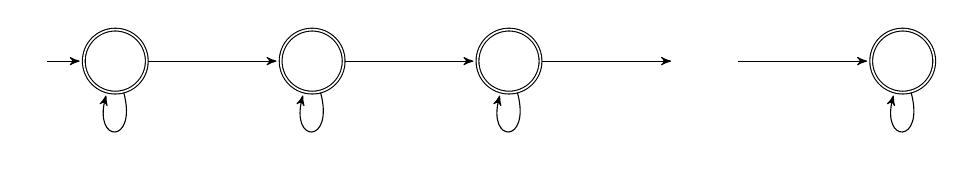
\begin{tikzpicture}[shorten >=1pt,node distance=2.5cm,
		on grid,>=stealth',initial text=,
		every state/.style={inner sep=2pt, minimum size=.8cm},
		 phantom/.style={draw=white},font=\footnotesize]
	\node[state,initial,accepting] (q0) {};
	\node[state,accepting] (p1) [right=of q0] {};
	\node[state,accepting] (p2) [right=of p1] {};
	\node[state,phantom] (p3) [right=of p2] {};
	\node[state,accepting] (p4) [right=of p3] {};

	\path[->] (q0) edge node [below] {}
                node [above] {} (p1)
            edge [loop below] node {} ()
		 (p1) edge node [below] {}
				node [above] {} (p2)
			edge [loop below] node {} ()
		(p2) edge node [below] {}
				node [above] {} (p3)
			edge [loop below] node {} ()
		(p3) edge node [below] {}
				node [above] {} (p4)
		(p4) edge [loop below] node {} ();
\end{tikzpicture}
\parbox{4.3in}{\caption{An input-preserving transducer realizing the channel . Each edge label  represents many transitions, one for each symbol  of the alphabet, and similarly for  and . Each edge label  represents
many transitions, one for each pair of distinct symbols
 and  from the alphabet. Thus, if the alphabet size is , then the size of the transducer is , as , or simply  if  is fixed.}\label{fig:inprestrans}}
\end{figure}


\begin{corollary}\label{th:ed}
Algorithm \texttt{DistErrDetect} computes the
edit distance of a language given via an NFA  in time 
where  is the cardinality of the alphabet used in .
\end{corollary}
\begin{proof}
For the correctness of the algorithm, first note that the loop in step 3 is set up such that 
is always error-detecting for . Also, based on the observations listed in the above remark, if  is error-detecting for  but not for
, then the desired distance
must be greater than  and at most , hence equal
to .
\pnsi
For the time complexity, the while loop will
perform  iterations. In each
iteration, the value  is
used to construct the transducer of
size  shown in Fig.~\ref{fig:inprestrans} with alphabet
being the set of alphabet symbols appearing
in the description of . Then, the transducer
 is constructed and its functionality
is tested in time .
As , it follows that the total time complexity is
as required.
\end{proof}

We note that, in the worst case,  is
of order  and, assuming a fixed alphabet, the above algorithm operates in time

which  is asymptotically better
than the time complexity stated in \cite{Kon:2007} when the
given automaton is an NFA.

\pssi
Next we present
the error-correction-based algorithm for estimating
the desired edit distance.

\begin{figure}[ht]
\begin{tabbing}
PAR \= No \= No \= NN \= \kill
\> Algorithm \texttt{DistErrCorrect} \\
\> 0.\> Input: NFA  \hspace{4mm} \\
\> 1.\> Let  be the bound in Lemma~\ref{lem:bound}\\
\> 2.\> Let  and \\
\> 3.\> Perform binary search to find  the largest  in
       \\
\>  \> for which  is error-correcting for  as follows: \\
\>  \>  \textbf{while} ()\\
\>  \>  a)\> Let \\
\>   \> b)\> Construct a transducer  realizing the channel \\
\>   \> c)\> Construct the transducer \\
\>   \> d)\> If ( is functional)  let \\
\>   \> \>  Else  let \\
\> 4. \>  \textbf{return} 
\end{tabbing}
\end{figure}

\begin{corollary}\label{cor:ec}
Algorithm \texttt{DistErrCorrect} returns
two values, differing by 1, one of which is the edit distance of
the language given via , in time   
where  is the cardinality of the alphabet used in .
\end{corollary}
\begin{proof}
For the correctness of the algorithm, first note that the loop in step 3 is set up such that 
is always error-correcting for . Also, based on the observations listed in the above remark, if  is error-correcting for  but not for
, then the desired distance
must be greater than  and at most , hence equal
to , or . Moreover, as ,
the initial value of  in step 2 is correct.
\pnsi
For the time complexity, the while loop will
perform  iterations. In each
iteration, the value  is
used to construct the transducer of
size  shown in Fig.~\ref{fig:inprestrans} with alphabet
being the set of alphabet symbols appearing
in the description of . Then, the transducer
 is constructed and its functionality
is tested in time .
As , it follows that the total time complexity is
as required.
\end{proof}
As noted before, in the worst case,  is
of order  and, assuming a fixed alphabet, the above algorithm operates in time

This time complexity is asymptotically better than the one in \cite{Kon:2007} even when the given automaton is a DFA.



\section{An  algorithm for edit distance via input-altering transducers}\label{sec:iat}
In this section we present a new (exact) method for computing much faster the desired edit distance via input-altering transducers---see theorem~\ref{th:final} and the associated algorithm.
A transducer  is called \emph{input-altering}, if

that is, the output of  is never equal to the input used. The new method is based on the following two major observations.
\begin{description}
  \item[(4.1)] The new result (see theorem~\ref{th:iat:ed}) that the property of error-detection for the channel  can be described via an input-altering transducer  of size .
  \item[(4.2)] The new observation that, using an input-altering transducer in our algorithms, eliminates the need for a binary search loop that builds a new transducer in each iteration. Instead, this loop can be replaced with the incremental construction of an NFA , which depends on , until a certain condition is satisfied, in which case the value of  is the desired edit distance---see further below for details.
\end{description}
The above observations are presented in two subsections.

\subsection{An input-altering transducer for error-detection}
We give first a quick summary of some concepts discussed
in \cite{DudKon:2012}.

\begin{remark}\label{rem:iat}
Let  be an input-altering transducer. The \emph{property
 described by}  is the set of all languages  satisfying

As explained in \cite{DudKon:2012}, this concept constitutes a formal method for specifying certain code properties defined via abstract
binary relations \cite{Shyr:Thierrin:relations}, and allows one to decide efficiently the
\emph{property satisfaction problem} by testing
condition~(\ref{eq:inpalt}). In particular, condition~(\ref{eq:inpalt}) can be tested
in time

where  is the NFA accepting the language 
and  is the input-altering transducer
describing the property for which  is to be tested.
This approach has led to the development of an
online language  server, called I-LaSer \cite{ilaser}.
\end{remark}

We shall show (see theorem~\ref{th:iat:ed}) that error-detection for  is definable via the input-altering transducer
, which is shown in Fig.~\ref{fig:inaltertrans} and
defined next.
The value  in a state  or  is called the {\em error counter}, meaning that any path from  to a state with error counter  has to be labeled  such that .
More precisely, we will define the edges such that a state  can be reached from  via a path with label   if and only if  for some word  and , thus,  is a proper prefix of  and state  remembers the left-most letter of  that occurs after its prefix .
A state  with  can only be reached via a path labeled  from  if
, thus, .
Furthermore, we make sure that for  such that neither  nor  there is a path from  to  which is labeled by  or .



\begin{figure}[ht]
\centering
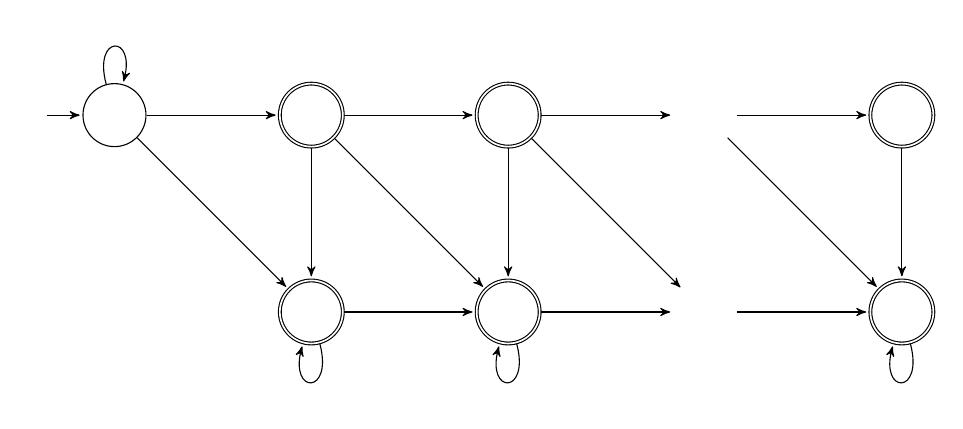
\begin{tikzpicture}[shorten >=1pt,node distance=2.5cm,
		on grid,>=stealth',initial text=,
		every state/.style={inner sep=2pt, minimum size=.8cm},
		 phantom/.style={draw=white},font=\footnotesize]
	\node[state,initial] (q0) {};
	\node[state,accepting] (q1) [right=of q0] {};
	\node[state,accepting] (q2) [right=of q1] {};
	\node[state,phantom] (q3) [right=of q2] {};
	\node[state,accepting] (q4) [right=of q3] {};

	\node[state,accepting] (p1) [below=of q1] {};
	\node[state,accepting] (p2) [right=of p1] {};
	\node[state,phantom] (p3) [right=of p2] {};
	\node[state,accepting] (p4) [right=of p3] {};

	\path[->] (q0) edge node [above] {} (q1)
			edge [loop above] node {} ()
			edge node [sloped,above] {} (p1)
		(q1) edge node [above] {} (q2)
			edge node [sloped,above] {} (p1)
			edge node [sloped,above] {}
				node [sloped,below] {} (p2)
		(q2) edge node [above] {} (q3)
			edge node [sloped,above] {} (p2)
			edge node [sloped,above] {}
				node [sloped,below] {} (p3)
		(q3) edge node [above] {} (q4)
			edge node [sloped,above] {}
				node [sloped,below] {} (p4)
		(q4) edge node [sloped,above] {} (p4)
		(p1) edge node [below] {}
				node [above] {} (p2)
			edge [loop below] node {} ()
		(p2) edge node [below] {}
				node [above] {} (p3)
			edge [loop below] node {} ()
		(p3) edge node [below] {}
				node [above] {} (p4)
		(p4) edge [loop below] node {} ();
\end{tikzpicture}
\parbox{4.3in}{\caption{A segment of the
input-altering transducer : for each  the complete transducer has  states of the form .
The labels  and  on an edge mean: one edge for each  with ; for some edge sets additional restrictions apply denoted, for example, by .}\label{fig:inaltertrans}}
\end{figure}

\begin{definition}\label{def:tr}
The transducer

is defined as follows. The set of states is

with all but the initial state  being final states: 
The edges in  can be divided into the four sets of edges .
The edges from  do not introduce any error, edges from the other sets model one substitution (), insertion (), or deletion ():

\end{definition}
\pmsn \textbf{Terminology}. If  is a transducer in standard form, then we write  for the NFA 
over the edit alphabet , where the labels of
the transitions in  are viewed as elements of . Note that, the label of a path  in  is a pair of words , whereas the label of the
corresponding path in , which we denote as , is an edit string
 such that  and .
This type
of NFA is called an eNFA in \cite{KaKo:2004}.


\begin{lemma}\label{lem:Adi:props}
Let  and let  be words. The following statements hold true with respect to the transducer .
\begin{enumerate}[i.)]
\item
In , every path from the start state  to any state  or  has as label a reduced edit string
whose weight is equal to .
\item
If  and  is a reduced edit string realizing , then
 is accepted by .
\item
If , then .
\item
If  and , for some symbol , then   .
\item
If  and , then .
\end{enumerate}
\end{lemma}
\begin{proof}
The \underline{first} statement follows when we note that the  definition of  and  implies the
following facts: (a) An edge exists between a state
with error counter  to one with error counter  ,
if and only if the label of that edge is an error;
thus, in any path from  to  or , the label of that path consists of exactly  errors.
(b) Any edit string accepted by  is indeed reduced.
\par
For the \underline{second} statement, consider any reduced edit string  realizing .
If the first error in  is a deletion, then  is of
the form
      
where each  is a non-error edit operation
of the form , 
is a deletion error,  and each  is
a deletion error, and  is an edit string that is
either empty
or starts with a non-deletion edit operation 
such that . If  is nonempty, then by definition of  the
following is a path

accepting . Similarly, a path accepting  exists in
 , if  is empty.
\par
Finally, one verifies that if the first error in 
is a substitution, then again  is accepted by .
\par
For the \underline{third} statement, if , then  is the label of a path  from 
to a final state  or , with . As the label of the path  has exactly  errors,
it follows that .
\par
 We also need to show that , that is, .
First consider the case where the path  ends at , with . Then,
the label of  is an edit string of the form

and  and .
Hence, . Now consider the case where the path  ends at state .
There are three cases. (a) The states used in the path are .
(b) The states used in  are , for some appropriate .
(c)  The states used in  are , for some appropriate .
In all three cases, one verifies that . For example, in case (b),  must be of the form
 and  of the form , where the
's are symbols,  are words, and  is a symbol other than ; hence,
.
\par
For the \underline{fourth} statement, let , with each  and  being a symbol,
and .
We use lemma~\ref{lem:didist}.
The edit string 
realizes . Moreover, this edit string is the label of a path in  from
 to . Hence, there is a path
in  from  to  with
label , as required.
\par
For the \underline{fifth} statement, let  be an edit string realizing . By definition
of , at each state of the form  with , one can follow an edge whose
label  can be of any of the
four types of edit operations, and moreover, if  is an error, then the edge goes into ,
that is, .
As  contains exactly  errors, there is a path from  to  whose label is made of the edit operations in . Hence, there is a path in  from  to  whose label is , as required.
\end{proof}


\begin{theorem}\label{th:iat:ed}
For each , the transducer  is input-altering and of size , and
describes the property of error-detection for the channel .
\end{theorem}
\begin{proof}
By construction, it follows that  is trim and has a number of states and transitions that is linear with respect to . Hence, it is indeed of size .
The third statement of lemma~\ref{lem:Adi:props} implies that the transducer is input-altering.
For the error-detection part, using the first statement of remark~\ref{rem:ed}, it is sufficient  to show that, for every language ,


First, for the `if' part, assume  and consider any words .  We need to
prove .
If  then this holds as  is input-altering. Else, it follows from the third statement of
lemma~\ref{lem:Adi:props}.  Now for the `only if' part, assume

but, for the sake of contradiction,  suppose there are different words  such that . If  is a prefix of , then
, for some , and
the fourth statement of the above lemma implies
 and, therefore, , which contradicts~(\ref{eq:iatp}).
By symmetry, a contradiction arises if  is a prefix of .

Now consider the case where  is not a prefix of  , and  is not a prefix of . Then,  and  for some words  and   symbols  with 
\emph{We shall obtain a contradiction
to (\ref{eq:iatp}) by showing the existence of a path , or , where  is a final state of }.
Let  be an edit string realizing
. Recall . As , the first edit operation, say  , of  must
be an error, that is, not of the form . Let . We consider three cases for .
First, if  is a substitution, then   and . By the fifth statement of the above lemma, . Then, the required path is


Now consider the case where . Then,  and  realizes . Let  be the number of deletions (if any) at the beginning of  so that any edit operation
following these deletions is not a deletion. Thus,  is of the form  with 
and , where  is a word of length , and
 and , for some word , and
,
and .
As  is nonempty, also  is nonempty, so let  be the first edit operation of , which
cannot be a deletion.
If , then  and  consists of insertions, and the required path is

If , then there is a symbol  such that .
If , then   cannot be a substitution, so it must be the non-error  or the insertion
. Then, the required path is

where  and  (case of ), or  and  (case of ).
If , then  must be the insertion  or the substitution . Again, in either case,
a path as required exists.

Finally, the case of , is symmetric to the previous one by simply switching the
roles of  and .
\end{proof}


\subsection{The  algorithm for edit distance}
Here we use the results of the previous subsection to arrive at an efficient algorithm for computing the desired
edit distance.
Remark~\ref{rem:iat}  and theorem~\ref{th:iat:ed}  imply that the \emph{intermediate} algorithm
\texttt{DistFirstInpAlter}
shown below correctly computes the desired edit distance. Moreover, by reasoning as in the proof of corollary~\ref{th:ed}, it follows that this algorithm executes in time , where  is the cardinality of the alphabet used in .


\begin{figure}[ht]
\begin{tabbing}
PAR \= No \= No \= NN \= NN \=\kill
\> Algorithm \texttt{DistFirstInpAlter} \\
\> 0.\> Input: NFA  \hspace{4mm} \\
\> 1.\> Let  be the bound in Lemma~\ref{lem:bound}\\
\> 2.\> Let  and  \\
\> 3.\> Perform binary search to find  the largest  in
       \\
\>  \> for which  is error-detecting for  as follows: \\
\>  \>  \textbf{while} ()\\
\>  \>  a)\> Let \\
\>   \> b)\> Construct the transducer  \\
\>   \> c)\> Construct NFA   accepting \\
\>   \> d)\> If ( accepts )  let \\
\>   \> \>  Else  let \\
\> 4. \> \textbf{return} 
\end{tabbing}
\end{figure}


We note again that, in the worst case,  is
of order  and, assuming a fixed alphabet, the above algorithm operates in time

which is asymptotically better than those of all other
known algorithms. However, we now discuss in detail the second major observation stated in the beginning of section~\ref{sec:iat}, which leads to the most efficient algorithm in theorem~\ref{th:final}. In particular, for the sake of clarity, we present that algorithm in two steps.
In the first place, we notice that the while loop
in \texttt{DistFirstInpAlter}
can be replaced with the construction
of the automaton  and a search
in that automaton for a path from the start state to
a final one in which the error counter value is minimal (this
value would be the required edit distance).
\begin{tabbing}
PAR \= No \= No \= NN \= NN \=\kill
\> Algorithm \texttt{DistNextInpAlter} \\
\> 0.\> Input: NFA  \hspace{4mm} \\
\> 1.\> Let  be the bound in Lemma~\ref{lem:bound}\\
\> 2.\> Construct the transducer  \\
\> 3.\> Construct NFA   accepting
        \\
\> 4.\> Starting at the start state of , use breadth first search (BFS) \\
\>   \> to visit all states. In doing so, keep track of the smallest\\
\>   \> error counter  in the visited final states of .\\
\> 5. \> \textbf{return} 
\end{tabbing}
As usual in product constructions, the states of  are triples of the form
, where  is a state of , and ,  are states of . The start state of  is
, where  is the start state of , and the final states of  are those triples consisting of final states in  and . A transition

exists in  if and only if the following transitions

exist in ,  and , respectively,
for some label , where  results if we add to
 empty  loop transitions  for all states
 in . The correctness of the above algorithm follows
from lemma~\ref{lem:Adi:props} and the definition of
. The breadth first search process requires time
linear with respect to the size of , which is

and this also is the time complexity of the above
algorithm (when the alphabet is fixed).
\par
The final improved algorithm results if we notice that
the desired edit distance can be much smaller
than  and that it can be computed
using only an `initial' part of .
In other words, one can first build  and
 accepting , and test whether  has any accepting path. If not, this
process is repeated by extending  to 
until some extended automaton, say , has an
accepting path, in which case the desired distance is
equal to .
\begin{tabbing}
PAR \= No \= No \= NN \= NN \=\kill
\> Algorithm \texttt{DistBestInpAlter} \\
\> 0.\> Input: NFA  \hspace{4mm} \\
\> 1.\> Construct the transducer  \\
\> 2.\> Construct NFA   accepting  \\
\> 3.\>  \\
\> 4. \>  \textbf{while} ( has no accepting path)\\
\>  \>  a)\> \\
\>   \> b)\>   \\
\> 5. \> \textbf{return} 
\end{tabbing}
The function \texttt{Extend} in the above algorithm works
based on the structure of  in Fig.~\ref{fig:inaltertrans} and is \emph{partially} shown below. For clarity,
we emphasize the fact that, in each step  of this algorithm, the final states of  are only
triples of the form  or , that is,
when , no triples of the form  or  are final states in .
\begin{tabbing}
PAR \= No \= No \= NN \= NN \=NN \=\kill
\> Function \texttt{Extend} (partial view)\\
\> let  be a copy of  \\
\> for each state of the form  in  \\
\> \> for each transitions  and  in  \\
\>\>\> if ( and )\\
\>\>\>\> add to  the transition \\
\>\>\>\> if  and  are final in  then
 is final in \\
\>\>\> if ( and )\\
\>\>\>\> add to  the transition \\
\>\>\>\> if  and  are final in  then
 is final in \\
\>\>\> \\
\> \textbf{return} the NFA 
\end{tabbing}
Based on the above discussion, the correctness of the following theorem has been established.
\begin{theorem}\label{th:final}
Algorithm \texttt{DistBestInpAlter} computes the
edit distance of the language given via an NFA  in
time , where  is the cardinality
of the alphabet used in  and  is the
computed edit distance.
\end{theorem}



\section{Implementation and testing}\label{sec:implem}
We have implemented the main algorithm \texttt{DistBestInpAlter} of theorem~\ref{th:final}, as well as the intermediate versions
\pssi
\texttt{DistErrDetect, DistErrCorrect, DistFirstInpAlter,}
\pssn
using the FAdo library for automata
\cite{Fado}, which is well maintained and provides
several useful tools for manipulating automata.
Moreover, we have used some of the implementations
of I-LaSer \cite{ilaser} involving product constructions
between transducer and automaton objects of the FAdo
library. We note that an implementation in C++ of the
algorithm in \cite{Kon:2007} is discussed in
\cite{Daka:2011}, but the execution time is too slow
to be used for any meaningful comparisons with the algorithms
presented here. Our best algorithm can be executed online
at \cite{olaser}. The user can enter as input
an NFA in Grail or FAdo format, select the algorithm to execute,
and press the Submit button.

We have performed several
tests\footnote{All tests were performed on a machine with the
following specification.
  Make: Acer,
  CPU: AMD Athlon(tm) II X2 215,
  Clock speed: 2.70 GHz,
  Memory (RAM): 4.00 GB,
  Operating System: Windows 7 64-bit.}
for the correctness
of these algorithms, as well as two sets of tests for the time complexity, which confirm  the theoretical
result that \texttt{DistBestInpAlter}
is indeed the fastest algorithm. We note that, for the
other three algorithms, we have skipped the step of
computing the upper bound  on the edit distance,
as this step is the same for all these algorithms, thus
resulting in faster execution without affecting in any
essential way the performance comparisons.

The two sets of tests correspond to two sequences of
automata  and , shown in the next two figures, for which we used  as the value of .
The first test set is such that the desired distance is equal to , for each NFA , that is, the distance grows
with  and, in fact, it is a worst-case scenario where the
distance is equal to the number of states of the NFA.
The second test set is such that the desired distance is fixed, equal to 2,
for all .
\begin{figure}[ht]
\centering
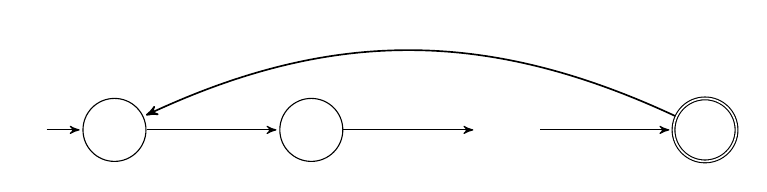
\begin{tikzpicture}[shorten >=1pt,node distance=2.5cm,
		on grid,>=stealth',initial text=,
		every state/.style={inner sep=2pt, minimum size=.8cm},
		 phantom/.style={draw=white},
to/.style={->,>=stealth',shorten >=1pt,semithick,font=\sffamily\footnotesize},
        font=\footnotesize]
	\node[state,initial] (q0) {};
	\node[state] (p1) [right=of q0] {};
	\node[state,phantom] (p2) [right=of p1] {};
	\node[state,accepting] (p3) [right=of p2] {};

	\path[->] (q0) edge node [below] {} (p1)
		 (p1) edge node [below] {} (p2)
		 (p2) edge node [below] {} (p3);
    \draw[to]
		(p3) to[bend right=25] node[midway,below] {}
        (q0);
\end{tikzpicture}
\parbox{4.3in}{\caption{The automaton  accepting the language .}\label{fig:testA}}
\end{figure}


\begin{figure}[ht]
\centering
\begin{tikzpicture}[shorten >=1pt,node distance=1.5cm and 1.5cm,
		on grid,>=stealth',initial text=,
		every state/.style={inner sep=2pt, minimum size=1cm},
		phantom/.style={draw=white},
		to/.style={->,>=stealth',shorten >=1pt,semithick,font=\sffamily\footnotesize},
        font=\footnotesize]
	\node[state,initial] (q0) {};
	\node[state,phantom] (q1) [above right=of q0] { };
	\node[state,phantom] (q2) [below right=of q0] { };
	\node[state,phantom] (q3) [right=of q0] {};

	\node[state] (p0) [right=of q3] {};
	\node[state] (p1) [above right=of p0] {};
	\node[state,phantom] (p11) [above right=of p1] { };
	\node[state,phantom] (p12) [below right=of p1] { };
	\node[state] (p2) [below right=of p0] {};
	\node[state,phantom] (p21) [above right=of p2] { };
	\node[state,phantom] (p22) [below right=of p2] { };
	\node[state,phantom] (p3) [right=of p1] {};
	\node[state,phantom] (p4) [right=of p2] {};

	\node[state] (r1) [right=of p3] {};
	\node[state] (r2) [right=of p4] {};
	\node[state,accepting] (r3) [below right=of r1] {};

	\path[->]
		(q0) edge node [below,sloped] {} (q1)
			 edge node [above,sloped] {} (q2)
		(p0) edge node [below,sloped] {} (p1)
			 edge node [above,sloped] {} (p2)
		(p1) edge node [below,sloped] {} (p11)
			 edge node [above,sloped] {} (p12)
		(p2) edge node [below,sloped] {} (p21)
			 edge node [above,sloped] {} (p22)
		(r1) edge node [below,sloped] {} (r3)
		(r2) edge node [above,sloped] {} (r3);

\end{tikzpicture}
\parbox{4.3in}{\caption{The automaton  with  states, where
. The states are 
and , with  and .
This automaton accepts the Levenshtein code consisting of all binary words  of length  such that , where `\%' is the integer division remainder operation. This code has edit distance equal to 2. On the other hand, its distance for insertion/deletion errors only is 3, so it is error-correcting for the 1-insertion/deletion per word channel.}\label{fig:testB}}
\end{figure}
The next table shows the actual running times of the
four algorithms on the NFAs
.
The number in parentheses next to each  indicates the number of states in .

\pmsi
\begin{tabular}{|c|c|c|c|c|}\hline
NFA & ErrDetection & ErrCorrection  &  FirstInpAlter
& BestInpAlter\\  \hline
 &  3.94s & 0.35s & 0.08s & 0.008s  \\  \hline
 & 19.20s & 0.48s & 0.11s & 0.010s  \\  \hline
 & 107.35s & 2.54s & 0.18s & 0.013s  \\  \hline
 & 442.01s & 4.03s & 0.33s & 0.016s  \\  \hline
 &  & 144.75s & 1.31s & 0.020s  \\  \hline
 &  & 12475.27s & 10.21s & 0.029s  \\  \hline
 &  &  & 46.28s & 0.109s  \\  \hline
\end{tabular}
\pbsn
The next table shows the actual running times of the
four algorithms on the NFAs .
The number in parentheses next to each  indicates the number of states in .
\pmsi
\begin{tabular}{|c|c|c|c|c|}\hline
NFA & ErrDetection & ErrCorrection  &  FirstInpAlter
& BestInpAlter\\  \hline
 & 0.889s & 0.164s & 0.098s & 0.027s  \\  \hline
 & 212.32s & 7.06s & 0.655s & 0.039s  \\  \hline
 &  & 72.25s & 4.63s & 0.097s  \\  \hline
 &  & 3806.74s & 40.79s & 0.234s  \\  \hline
 &  &  & 375.17s & 0.735s  \\  \hline
 &  &  & 2070.21s & 1.919s  \\  \hline
\end{tabular}
\pbsn
Let  be the computed edit distance in the above test
sets.
The best algorithm has about the same performance in both test cases, even though  is a parameter in its time complexity .
A possible explanation is that the NFA  has more edges than those of , when both  and  have the same number of states.
A reason why the intermediate algorithms perform a lot better on   than on  with the same number of states is that the value of the edit distance upper bound
in  is smaller than that in .
\pbsn
A further improvement to our algorithms, to be implemented, is that one can
remove from Fig.~\ref{fig:inaltertrans} all the diagonal transitions
from a state  to a state . This is because,
for any edit string of the form

accepted by , where  and
the 's are non-errors, the
automaton  also accepts

such that , , and
. Moreover  accepts
 using none of the diagonal transitions that are
to be removed as specified above.
A similar observation holds if we replace in  the edit
operation  shown in  with ,
where .
Of course this improvement does not affect in any significant
way the performance comparisons among the four algorithms.


\section{Conclusion}\label{sec:last}
This paper represents a significant improvement in  the
time complexity of computing the edit distance of a given regular language.
As discussed in \cite{Kon:2007}, this problem is related to
the inherent capability of a language to detect substitution,
insertion, and deletion errors. The method based on using the input-altering transducer 
seems to adapt to other types of errors as well.
For example, one can construct a similar input-altering transducer for insertion/deletion only errors. It seems
promising to investigate the problem when the errors
have different costs (in the current setting, the cost of
each error is 1).

The present contribution stemmed from the
question of whether the error-detection property for
the channel   can be described by an
input-altering transducer. The more general question
of whether an input-preserving transducer property of
interest can be described by an input-altering transducer is important to investigate, as this would lead to more
efficient algorithms for deciding the property
satisfaction problem (whether, given a regular language
and a transducer property, the language satisfies the property).





\bibliographystyle{abbrv}
\bibliography{refs}

\end{document}
